\chapter{Introducción a las cadenas de Markov}
En este capítulo vamos a inicializar la teoría de cadenas de Markov, avanzado progresivamente hacia las cadenas de Markov ocultas. En primer lugar, vamos a presentar el concepto de procesos de Markov:

\section{Propiedad de Markov}
Sea $\mathbb{S}$ un conjunto finito de forma $\{s_1,...,s_n\}$, definimos un proceso estocástico sobre $\mathbb{S}$ como una secuencia de variables aleatorias $\{\mathcal{X}_0,\mathcal{X}_1,\mathcal{X}_2,...\}$, o $\{\mathcal{X}_t\}_{t=0}^{\infty}$ para acortar, donde cada $\mathcal{X}_t$ es una variable aleatoria que toma valores en $\mathbb{S}$.


 A pesar de que el índice $t$ puede representar cualquiera magnitud, lo más común es que represente el tiempo. Si tomamos el índice $t$ como el tiempo, obtenemos la noción de \enquote{pasado} y \enquote{futuro}, esto es, si $t<t'$, entonces $\mathcal{X}_t$ es una variable \enquote{pasada} para $\mathcal{X}_{t'}$, mientras que $\mathcal{X}_{t'}$ es una variable \enquote{futura} para $\mathcal{X}_t$. Sin embargo, esto no es siempre así, por ejemplo, si el proceso estocástico corresponde al de las secuencias de genomas de un organismo, el conjunto $\mathbb{S}$ estará formado por los cuatro símbolos para las subunidades de nucleótidos $\{A,C,G,T\}$ y las secuenciaciones tienen un significado más espacial que temporal.
 
\begin{definition}
Un proceso estocástico $\{\mathcal{X}_t\}_{t=0}^{\infty}$ se dice que posee \textbf{la propiedad de Markov}, o es un \textbf{proceso de Markov}, si para todo $t\geq1$ y $(u_0,...,u_{t-1},u_t)\in\mathbb{S}^{t+1}$ se tiene que:
\[ \tag{1.\arabic{CadeanasMarkov}}\label{eqDefMarkov}
    P[\mathcal{X}_t=u_t|\mathcal{X}_0=u_0,...,\mathcal{X}_{t-1}=u_{t-1}]=P[\mathcal{X}_t=u_t|\mathcal{X}_{t-1}=u_{t-1}]
\]
\end{definition}

La propiedad de Markov afirma que las distribuciones condicionadas del \enquote{estado actual} $\mathcal{X}_t$ depende únicamente del \enquote{pasado inmediato} $\mathcal{X}_{t-1}$ y no depende de ninguno de los anteriores estados. 

Por conveniencia, introducimos la notación $\mathcal{X}_j^k$ para denotar los estados $\mathcal{X}_i$ con $j\leq i\leq k$. Con esta notación, podemos reescribir la Definición 1.1 como sigue: Un proceso estocástico $\{\mathcal{X}_t\}$ es un \textbf{proceso de Markov} si, para todo $(u_0,...,u_{t-1},u_t)\in\mathbb{S}^{t+1}$ es cierto que:
\[  \stepcounter{CadeanasMarkov}
    \tag{1.\arabic{CadeanasMarkov}}\label{eqDefMarkov2}
    P[\mathcal{X}_t=u_t|\mathcal{X}_0^{t-1}=u_0...u_{t-1}]=P[\mathcal{X}_t=u_t|\mathcal{X}_{t-1}=u_{t-1}]
\]

Para cualquier proceso estocástico $\{\mathcal{X}_t\}$ y cualquiera secuencia $(u_0,...,u_{t-1},u_t)\in\mathbb{S}^{t+1}$, tenemos que por definición de probabilidad condicionada:

\[
P[\mathcal{X}_0^t=u_0...u_t]=P[\mathcal{X}_0=u_0]\cdot\prod_{i=0}^{t-1}P[\mathcal{X}_{i+1}=u_{i+1}|\mathcal{X}_0^i=u_0...u_i]
\]

Sin embargo, si consideramos un proceso de Markov, entonces la fórmula anterior se reduce a:
\[ \stepcounter{CadeanasMarkov}
\tag{1.\arabic{CadeanasMarkov}} \label{propiedadMarkov}
P[\mathcal{X}_0^t=u_0...u_t]=P[\mathcal{X}_0=u_0]\cdot\prod_{i=0}^{t-1}P[\mathcal{X}_{i+1}=u_{i+1}|\mathcal{X}_i=u_i]
\]

En probabilidad, es usual referirse con el nombre \textbf{cadena de Markov} a un proceso de Markov $\mathcal{X}_t$ donde el parámetro $t$ toma únicamente valores discretos. En este trabajo, pondremos nuestra atención en los casos donde $t$ toma valores en $\mathbb{N}_0$.

En (\ref{propiedadMarkov}) vemos la importancia del valor:
\[
P[\mathcal{X}_{t+1}=u|\mathcal{X}_t=v]
\]

al que podemos identificar como una función de tres variables: el estado \enquote{actual} $v\in\mathbb{S}$, el estado \enquote{siguiente} $u\in\mathbb{S}$ y el \enquote{tiempo actual} $t\in\mathbb{N}_0$. Así, teniendo en cuenta que $\mathbb{S}=\{s_1,...,s_n\}$ definimos para todo tiempo $t\in\mathbb{N}_0$ la probabilidad de transición:

\[ \stepcounter{CadeanasMarkov}
\tag{1.\arabic{CadeanasMarkov}} \label{compTransición}
a_{ij}(t):=P[\mathcal{X}_{t+1}=s_j|\mathcal{X}_t=s_i]
\]

Por tanto, $a_{ij}(t)$ es la probabilidad de realizar una transición desde el estado actual $s_i$ al estado siguiente $s_j$ en el instante $t$.

\begin{definition}
Sea $\mathcal{X}_t$ una cadena de Markov, la matriz cuadrada de dimensión $n$,  $A(t)=[a_{ij}(t)]$, es la \textbf{matriz de transición} de $\mathcal{X}_t$ en el instante $t$. Una cadena de Markov es \textbf{homogénea} si $A(t)$ es constante para todo $t\in\mathbb{N}_0$, en otro caso, es \textbf{no homogénea}. 
\end{definition}

\begin{definition}
Sea $\mathcal{X}_t$ una cadena de Markov tomando valores en un conjunto finito $\mathbb{S}=\{s_1,...,s_n\}$, y sea $A(t)$ su matriz de transición en el instante $t$. Entonces, $A(t)$ es una \textbf{matriz estocástica} (por filas) para todo $t$, esto es:
\begin{align*}
a_{ij}(t)\in[0,1],\, \forall i,j \in \{1,...,n\}, t\in\mathbb{N}_0\\
\sum_{j=1}^n a_{ij}(t)=1, \, \forall i\in\{1,...,n\}, t\in\mathbb{N}_0
\end{align*}
\end{definition}

\begin{proposition}\label{propiedadMatrizEstocástica}
    
Sea $A$ una matriz positiva (cuyos elementos son no negativos, con al menos un elemento estrictamente positivo) de dimensión $n\times n$:
\begin{enumerate}
    \item $A$ es estocástica si y solo si 1 es un valor propio de $A^T$ con vector propio (a la izquierda) $\mathbf{1}=\begin{pmatrix}1 & 1 & \dots & 1\end{pmatrix}$.
    \item si $A$ es estocástica, entonces para todo valor propio $\lambda$, se cumple que  $\left|\lambda\right|\leq1.$
\end{enumerate}
\end{proposition}

\begin{proofs*}
\
\begin{enumerate}
    \item Es suficiente con observar que la condición de estocaticidad para una matriz positiva $A$ es equivalente a que $\mathbf{1}\cdot A^T=\mathbf{1}$.
    \item Sea $v$ un vector propio asociado (a izquierda pues estamos usando la notación fila) a $\lambda$, por ser $A$ positiva y estocástica, tenemos que:
    \[
    \left|\lambda\right|\sum_{j=1}^n\left| v_j\right|=\sum_{j=1}^n\left|\lambda v_j\right|= \sum_{j=1}^n\left|(vA)_j \right|  =\sum_{j=1}^n\left|\sum_{i=1}^n a_{ij}v_i\right|\]
    \[\leq\sum_{j=1}^n\sum_{i=1}^n a_{ij}\left|v_i\right|=\sum_{i=1}^n\left( \sum_{j=1}^n a_{ij} \right) \left|v_i\right|=\sum_{i=1}^n\left|v_i\right|\]
    Puesto que $\sum_{r=1}^n\left|v_r\right|\neq0$, tenemos que $\left|\lambda\right|\leq1$.\qed
\end{enumerate}
\end{proofs*}

\begin{remark}\label{productoEstocásticos}
De la primera afirmación de la proposición \ref{propiedadMatrizEstocástica}, podemos ver que el producto de matrices estocásticas sigue siendo estocástica. En efecto, si $A, B$ son dos matrices estocásticas entonces $\mathbf{1}\cdot\left(AB\right)^T=\mathbf{1}\cdot B^T\cdot A^T=\mathbf{1}\cdot A^T=\mathbf{1}$.
\end{remark}
Para continuar con los estudios de las cadenas de Markov presentamos el siguiente conjunto:

\begin{definition}
El \textbf{n-símplex estándar} es el subconjunto de $\mathbb{R}^{n+1}$ dado por:
\[
\Delta^n=\{(t_1,...,t_{n+1})\in \mathbb{R}^{n+1} \, |\, \sum_{i=1}^{n+1} t_i=1 \text{ y } t_i\geq0 \text{ para todo } i\}
\]
\end{definition}
Puesto que para todo $t$, $\sum\limits_{i=1}\limits^n P[\mathcal{X}_t={s_i}]=1$; para cada instante, podemos representar las probabilidades de que la cadena se encuentre en cada estado con un vector de $\Delta^{n-1}$.

\begin{theorem}

Sea $\{\mathcal{X}_t\}$ una cadena de Markov con valores en $\mathbb{S}=\{s_1,...,s_n\}$, y sea $A(t)$ su matriz de transición en el instante $t$. Supongamos que $\mathcal{X}_0$ se distribuye de acuerdo con $c^0 \in \Delta^{n-1}$, esto es:
\[
P[\mathcal{X}_0=s_i]=c_i^0,\, \forall i \in \{1,...,n\}
\]
Entonces, para todo $t\geq0$, $\mathcal{X}_t$ se distribuye de acuerdo con:
\[\stepcounter{CadeanasMarkov}
\tag{1.\arabic{CadeanasMarkov}} \label{fórmulaDistribuciónEnT}
c^t=c^0A(0)A(1)\cdot\cdot\cdot A(t-1)
\]
\end{theorem}

\begin{proofs*}
Sea $s_i\in \mathbb{S}$, por \ref{propiedadMarkov} tenemos que:

\[P[\mathcal{X}_t=s_i]=\]
\[\sum_{u_0u_1...u_{t-1}\in\mathbb{S}^{t}}P[\mathcal{X}_0=u_0]\cdot\prod_{i=0}^{t-2}P[\mathcal{X}_{i+1}=u_{i+1}|\mathcal{X}_i=u_i]\cdot P[\mathcal{X}_t=s_i|\mathcal{X}_{t-1}=u_{t-1}] \]
\[=\sum_{u_0u_1...u_{t-1}\in\mathbb{S}^{t}}c_{u_0}\cdot a_{u_0,u_1}(0)\cdot\cdot\cdot a_{u_{t-2},u_{t-1}}(t-2)\cdot a_{u_{t-1},s_i}(t-1)\]
Notemos que esta última expresión es justamente la componente $i$-ésima de $c^t=c^0A(0)A(1)\cdot\cdot\cdot A(t-1)$ escrita en forma extensa.\qed
\end{proofs*}

\begin{exampleth}
En este ejemplo presentamos una variación del juego de cartas \enquote{blackjack}. En este caso, tenemos un dado de cuatro caras con valores 0, 1, 2 y 3, y con probabilidad uniforme en cada lanzamiento. Un jugador lanza el dado de forma repetida y $\mathcal{X}_t$ representa el valor acumulado tras $t$ lanzamientos. Si el total es igual a nueve, el jugador gana; en otro caso se considera que pierde. Podemos asumir que el resultado de cada lanzamiento es independiente de los lanzamientos anteriores.

Tenemos entonces que $\{\mathcal{X}_t\}$ toma valores en el conjunto $\mathbb{S}:=\{0,1,...,8,W,L\}$ de cardinalidad 11. Sea $\mathcal{Y}_t$ el resultado del lanzamiento en el instante $t$:
\[
P[\mathcal{Y}_t=0]=P[\mathcal{Y}_t=1]=P[\mathcal{Y}_t=2]=P[\mathcal{Y}_t=3]=1/4
\]

Examinemos ahora la distribución de $\mathcal{X}_t$, por definición sabemos que $\mathcal{X}_t=\mathcal{X}_{t-1}+\mathcal{Y}_t$, excepto el caso de que $\mathcal{X}_{t-1}+\mathcal{Y}_t=9$, consideraremos $\mathcal{X}_t=W$ (ganar); y si $\mathcal{X}_{t-1}+\mathcal{Y}_t>9$, consideraremos $\mathcal{X}_t=L$ (perder). Si $\mathcal{X}_{t-1}=W$ o $L$, consideraremos que el juego está acabado y $\mathcal{X}_t=\mathcal{X}_{t-1}$. Estas observaciones se pueden resumir en las siguientes reglas:

\begin{itemize}
    \item Si $\mathcal{X}_{t-1}\leq5$:
    \[
    P[\mathcal{X}_t=\mathcal{X}_{t-1}]=P[\mathcal{X}_t=\mathcal{X}_{t-1}+1]=\]\[=P[\mathcal{X}_t=\mathcal{X}_{t-1}+2]=P[\mathcal{X}_t=\mathcal{X}_{t-1}+3]=1/4
    \]
    \item Si $\mathcal{X}_{t-1}=6$:
    \[
    P[\mathcal{X}_t=6]=P[\mathcal{X}_t=7]=P[\mathcal{X}_t=8]=P[\mathcal{X}_t=W]=1/4
    \]
    \item Si $\mathcal{X}_{t-1}=7$:
    \[
    P[\mathcal{X}_t=7]=P[\mathcal{X}_t=8]=P[\mathcal{X}_t=W]=P[\mathcal{X}_t=L]=1/4
    \]
    \item Si $\mathcal{X}_{t-1}=8$:
    \[
        P[\mathcal{X}_t=8]=P[\mathcal{X}_t=W]=1/4
    \]\[
        P[\mathcal{X}_t=L]=1/2
    \]
    \item Si $\mathcal{X}_{t-1}=W$ o $L$:
    \[
        P[\mathcal{X}_t=\mathcal{X}_{t-1}]=1
    \]
\end{itemize}

$\{\mathcal{X}_t\}$ es una cadena de Markov pues la distribución de $\mathcal{X}_t$ depende únicamente del valor de $\mathcal{X}_{t-1}$ y no de cómo se ha alcanzado dicho valor. Notemos que las probabilidades anteriores no dependen de $t$, con lo cual la matriz de transición de $\mathcal{X}_t$ es una matriz fija y $\mathcal{X}_t$ es homogénea. 

La matriz de transición de $\mathcal{X}_t$ es entonces una matriz 11$\times$11 dado por:

\begin{center}
    $A=\begin{pmatrix}
    1/4 & 1/4 & 1/4 & 1/4 & 0 & 0 & 0 & 0 & 0 & 0 & 0 \\   
    0 & 1/4 & 1/4 & 1/4 & 1/4 & 0 & 0 & 0 & 0 & 0 & 0 \\
    0 & 0 & 1/4 & 1/4 & 1/4 & 1/4 & 0 & 0 & 0 & 0 & 0 \\
    0 & 0 & 0 & 1/4 & 1/4 & 1/4 & 1/4 & 0 & 0 & 0 & 0 \\
    0 & 0 & 0 & 0 & 1/4 & 1/4 & 1/4 & 1/4 & 0 & 0 & 0 \\
    0 & 0 & 0 & 0 & 0 & 1/4 & 1/4 & 1/4 & 1/4 & 0 & 0 \\
    0 & 0 & 0 & 0 & 0 & 0 & 1/4 & 1/4 & 1/4 & 1/4 & 0 \\
    0 & 0 & 0 & 0 & 0 & 0 & 0 & 1/4 & 1/4 & 1/4 & 1/4 \\
    0 & 0 & 0 & 0 & 0 & 0 & 0 & 0 & 1/4 & 1/4 & 2/4 \\
    0 & 0 & 0 & 0 & 0 & 0 & 0 & 0 & 0 & 1 & 0 \\
    0 & 0 & 0 & 0 & 0 & 0 & 0 & 0 & 0 & 0 & 1 \\
    \end{pmatrix}$
\end{center}

Es natural que el juego comience con el valor inicial igual a cero. Por lo tanto, la distribución de $\mathcal{X}_0$ está representada por $c_0\in\mathbb{R}^{11}$ con un 1 en la primera componente y ceros en el resto. Aplicando repetidamente la fórmula \ref{fórmulaDistribuciónEnT} obtendremos las distribuciones de $\mathcal{X}_1,\,\mathcal{X}_2,$ etc. Así, sea $c_t$ la distribución de $\mathcal{X}_t$, tenemos:
\[
c_0=\begin{pmatrix}
1 & 0 & \dots & 0
\end{pmatrix}\]
\[
c_1=c_0A=\begin{pmatrix}
1/4 & 1/4 & 1/4 & 1/4 & 0 & \dots & 0
\end{pmatrix}\]
\[
c_2=c_1A=\begin{pmatrix}
1/16 & 1/8 & 3/16 & 1/4 & 3/16 & 1/8 & 1/16  & 0 & 0 & 0 & 0
\end{pmatrix}
\]

Cabe destacar que si examinamos la distribución $c_t$, entonces tenemos que $P[\mathcal{X}_t\in\{0\dots8\}]$ tiende a cero conforme $t\rightarrow\infty$. Esto es natural pues el juego terminará eventualmente en victoria ($W$) o en pérdida ($L$) y todos los otros estados son transitorias. Esta idea, nos introduce al siguiente apartado.

\end{exampleth}

\section{Estados de una cadena de Markov}
A partir de esta sección, vamos a centrarnos en el estudio de cadenas de Markov cuyas matrices de transición son constantes, en consecuencia, las probabilidades de transición son independientes del instante $t$. Nos referiremos a ellas directamente como cadenas de Markov, asumiendo homogeneidad. 

Está claro que los estados juegan un papel importante en el estudio de las cadenas de Markov, para describir con más detalles las propiedades de una cadena de Markov vamos a distinguir los estados que puede tener. Antes de empezar la clasificación, nos interesa saber cómo evoluciona una cadena de Markov tras $n$ instantes:


\begin{definition}
Sea $\{\mathcal{X}_t\}$ una cadena de Markov, $s_i, s_j \in \mathbb{S}$, $n,m\in\mathbb{N}_0$, denotamos:
\[P_{ij}^{m,m+n}:=P[\mathcal{X}_{n+m}=s_j|\mathcal{X}_m=s_i]\]
Si $n=0$:
\[P_{ij}^{m,m}=P[\mathcal{X}_{m}=s_j|\mathcal{X}_m=s_i]=\delta_{ij}=
\begin{cases}
    1, & \text{si } i=j\\
    0, &         \text{si } i\neq j
\end{cases}\]
\end{definition}
\begin{theorem}[Ecuación de Chapman-Kolmogorov]
En condiciones anteriores, sea $r\in \mathbb{N}_0$:
\[P_{ij}^{m,m+n+r}=\sum_{s_k\in\mathbb{S}}P_{ik}^{m,m+n}P_{kj}^{m+n,m+n+r}\]
\end{theorem}
\begin{proofs*}
    \[ P_{ij}^{m,m+n+r}=P[\mathcal{X}_{m+n+r}=s_j|\mathcal{X}_m=s_i]\]
    \[=\sum_{s_k\in\mathbb{S}} P[\mathcal{X}_{m+n+r}=s_j |\mathcal{X}_{m+n}=s_k,\mathcal{X}_m=s_i ] P[\mathcal{X}_{m+n}=s_k|\mathcal{X}_m=s_i ]\]
Aplicando la propiedad de Markov:
    \[P[\mathcal{X}_{m+n+r}=s_j |\mathcal{X}_{m+n}=s_k,\mathcal{X}_m=s_i ]\]\[=P[\mathcal{X}_{m+n+r}=s_j |\mathcal{X}_{m+n}=s_k]=P_{kj}^{m+n,m+n+r}\]
Por lo tanto:
    \[
    \pushQED{\qed}
    P_{ij}^{m,m+n+r}=\sum_{s_k\in\mathbb{S}}P_{ik}^{m,m+n}P_{kj}^{m+n,m+n+r}\qedhere
    \popQED\]
    
\end{proofs*}

Notemos que por ser $\{\mathcal{X}_t\}$, $P_{ij}^{m,m+1}$ es independiente de $m$, por lo cual aplicando inductivamente la ecuación de Chapman-Kolmogorov, tenemos que $P_{ij}^{m,m+n}$ son independientes de $m$. 
\begin{definition}
Sea $\{\mathcal{X}_t\}$ una cadena de Markov, $s_i, s_j \in \mathbb{S}$, $n,m\in\mathbb{N}_0$,  definimos las probabilidades de transición en $n$ pasos como:
\[a_{ij}^{(n)}:=P_{ij}^{m,m+n}=P[\mathcal{X}_{m+n}=s_j|\mathcal{X}_m=s_i]\]
Y la matriz de las probabilidades de transición en $n$ pasos como $A^{(n)}=[a_{ij}^{(n)}]$.
\end{definition}
\begin{lemma}
La matriz de transición en $n$ pasos cumple que $A^{(n)}=A^n, \forall n\in\mathbb{N}$. Por el comentario \ref{productoEstocásticos}, $A^{(n)}$ es estocástica.
\end{lemma}
\begin{proofs*}
 Expresando la ecuación de Chapman-Kolmogorov en forma matricial tenemos que $A^{(n+r)}=A^{(n)}A^{(r)}$, por ser $A^{(1)}=A$:
    \[
    \pushQED{\qed}
    A^{(n)}=A^{(n-1)}A=A^{(n-2)}A^2=\dots=A^n \qedhere
    \popQED\]    
\end{proofs*}

\subsection{Estados alcanzables y comunicables}
\begin{definition}
    El estado $s_j$ se dice \textbf{alcanzable} o \textbf{accesible} desde el estado $s_i$, representado por $i\longrightarrow j$, si existe $n\in\mathbb{N}_0$ tal que $a_{ij}^{(n)}>0$. Dos estados, $s_i$ y $s_j$, que son mutuamente alcanzables, se dicen \textbf{comunicables}, representado por $i\longleftrightarrow j$.
\end{definition}

La definición anterior tiene el significado siguiente: si $s_j$ es accesible desde el estado $s_i$, entonces existirá un $n\in\mathbb{N}_0$ tal que $P[\mathcal{X}_{m+n}=s_j]>0$ siempre que $\mathcal{X}_m=s_i$.  Es decir, empezando desde el estado $s_i$, hay una probabilidad positiva de que, en un número finito de transiciones, alcancemos el estado $s_j$.

\begin{theorem}
    La propiedad de comunicación, $\longleftrightarrow$, es una relación de equivalencia sobre el conjunto de estados $\mathbb{S}$.
\end{theorem}
\begin{proofs*}
    \
    \begin{itemize}
        \item $\textbf{Reflexividad: } a_{ii}^{(0)}=\delta_{ii}=1>0$. Por tanto, $i\longleftrightarrow i$.
        \item $\textbf{Simetría:}$ si $i\longleftrightarrow j$, existen $n,m\in\mathbb{N}_0$ tales que $a_{ij}^{(n)}, a_{ji}^{(m)}>0$, escogiendo los mismos $n$ y $m$, tenemos que $j\longleftrightarrow i$.
        \item $\textbf{Transitividad:}$ sean $i\longleftrightarrow j$ y $j\longleftrightarrow k$:
        \begin{itemize}
            \item Por ser $i\longleftrightarrow j$, existen $n,m\in\mathbb{N}_0$ tales que $a_{ij}^{(n)}, a_{ji}^{(m)}>0$.
            \item Por ser $j\longleftrightarrow k$, existen $r,s\in\mathbb{N}_0$ tales que $a_{jk}^{(r)}, a_{kj}^{(s)}>0$.
        \end{itemize}
        Aplicando entonces la ecuación de Chapman-Kolmogorov tenemos que:
        \begin{itemize}
            \item $a_{ik}^{(n+r)}=\sum\limits_{s_l\in\mathbb{S}}a_{il}^{(n)}a_{lk}^{(r)}\geq a_{ij}^{(n)}a_{jk}^{(r)}>0$
            \item $a_{ki}^{(s+m)}=\sum\limits_{s_l\in\mathbb{S}}a_{kl}^{(s)}a_{li}^{(m)}\geq a_{kj}^{(s)}a_{ji}^{(m)}>0$
        \end{itemize}
        Por lo tanto, $i\longleftrightarrow k$.\qed
    \end{itemize}
\end{proofs*}

Como resultado, podemos dividir el conjunto de los estados $\mathbb{S}$ en clases de equivalencias dependiendo de si existen comunicaciones entre los estados. Esto introduce a la siguiente definición:
\begin{definition}
    Sea $\{\mathcal{X}_t\}$ una cadena de Markov sobre un conjunto finito $\mathbb{S}$, $\{\mathcal{X}_t\}$ es \textbf{irreducible} si hay solo una clase de equivalencia sobre $\mathbb{S}$ mediante la relación $\longleftrightarrow$.
\end{definition}

Es decir, una cadena de Markov es irreducible si todos los estados se comunican unos con otros. Tomando el ejemplo de \enquote{blackjack}, podemos apreciar que:
    \begin{itemize}
        \item Un estado $s_i\in \{0\dots 8\}$ no es comunicable con un estado $s_j$ con valor inferior $\Longrightarrow a_{ij}^{(n)}=0, \forall n\in\mathbb{N}_0, j<i$.
        \item Los estados $W$ y $L$ no son modificables $\Longrightarrow a_{Wi}^{(n)}=a_{Li}^{(n)}=0, \forall n\in\mathbb{N}_0,  i \in \{0\dots 8, W$ o $L\}$
    \end{itemize}

Por simetría, cada estado es únicamente comunicable consigo mismo. En consecuencia, hay 11 clases de equivalencia en $\mathbb{S}$, uno por cada estado y la cadena de Markov no es irreducible.

\subsection{Periodicidad de una cadena de Markov}
\begin{definition}
Sea $a_{ii}^{(n)}$ la probabilidad de transición en $n$ pasos al estado $s_i$ desde $s_i$, el periodo $\lambda(i)$ de un estado $s_i$ es el máximo común divisor de todos los $n\in\mathbb{N}$ con $a_{ii}^{(n)}>0$, esto es:
\[
\lambda(i):=m.c.d(\{n\in\mathbb{N}\,|\, a_{ii}^{(n)}>0\})
\]
Si $a_{ii}^{(n)}=0$ para todo $n\in\mathbb{N}$, entonces definimos $\lambda(i):=0$.
\end{definition}
A continuación indicamos que la periodicidad también es una propiedad de clase. Esto es, si el estado $s_i$ en una clase tiene periodo $t$, entonces todos los estados de esa clase tienen periodo $t$.
\begin{theorem}
    Si $i\longleftrightarrow j$, entonces $\lambda(i)=\lambda(j)$, es decir, el periodo es constante en cada clase de equivalencia.
\end{theorem}
\begin{proofs*}
Si $i=j$ el resultado es trivial. Supongamos que $i\neq j$, entonces existen $n,m\in\mathbb{N}$ tales que $a_{ij}^{(n)},a_{ji}^{(m)}>0$, por la ecuación de Chapman-Kolmogorov:
\[ a_{ii}^{(n+m)}=\sum\limits_{s_l\in\mathbb{S}}a_{il}^{(n)}a_{li}^{(m)}\geq a_{ij}^{(n)}a_{ji}^{(m)}>0\Longrightarrow\lambda(i)\,|\,(n+m)\]
Sea $s\in\mathbb{N}$ tal que $a_{jj}^{(s)}>0$:
\[ a_{ii}^{(n+m+s)}\geq a_{ij}^{(n)}a_{jj}^{(s)}a_{ji}^{(m)}>0\Longrightarrow \lambda(i)\,|\,(n+m+s)\]
Por lo tanto, $\lambda(i)\,|\,s$, como $s$ es arbitrario, $\lambda(i)$ es un divisor común de $\{n\in\mathbb{N}\,|\, a_{jj}^{(n)}>0\}$, por definición de periodo, $\lambda(i)\,|\,\lambda(j)$. Realizando la misma discusión intercambiando los papeles de $i$ y $j$, obtenemos que $\lambda(j)\,|\,\lambda(i)$, por lo tanto, $\lambda(i)=\lambda(j)$. \qed
\end{proofs*}

\begin{definition}
Un estado $s_i$ se dice \textbf{no periódico} o \textbf{aperiódico} si $\lambda(i)=1$. 
\end{definition}
\begin{definition}
Una cadena de Markov se llama \textbf{no periódico} o \textbf{aperiódico} si todos sus estados son aperiódicos, de otra forma, \textbf{periódica}. Si la cadena de Markov es irreducible, entonces podemos hablar de \textbf{periodo de la cadena}.
\end{definition}
La periodicidad es una propiedad que se puede apreciar muy bien si representamos la cadena de Markov en forma de grafo. Veamos en el siguiente ejemplo:
\begin{exampleth}
Sea una cadena de Markov con la siguiente matriz de transición:
\begin{center}
    $A=\begin{pmatrix}
    0 & 1/2 & 0 & 1/2 \\
    0 & 0 & 1 & 0 \\
    1 & 0 & 0 & 0 \\
    0 & 0 & 1 & 0
    \end{pmatrix}$
\end{center}
Si representamos el grafo de estados:
    \begin{center}
        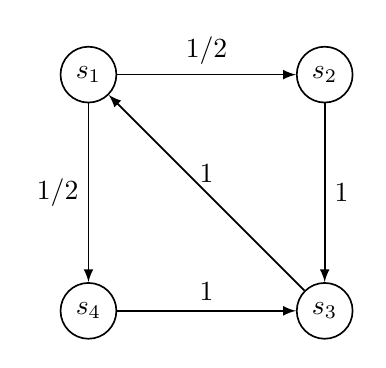
\begin{tikzpicture}[-latex ,auto , node distance =3 cm ,semithick,
        main/.style = {draw, circle}] 
            \node[main] (1) {$s_1$}; 
            \node[main] (2) [right of=1] {$s_2$};
            \node[main] (3) [below of=2] {$s_3$};
            \node[main] (4) [below of=1] {$s_4$};
            \draw (1) -- node[midway] {1/2} (2);
            \draw (1) -- node[midway,left] {1/2} (4);
            \draw (2) -- node[midway] {1} (3);
            \draw (3) -- node[midway,above] {1} (1);
            \draw (4) -- node[midway] {1} (3);
        \end{tikzpicture}
    \end{center}
Observando este grafo, podemos ver que todos los estados tienen periodo 3. Es más, todos los estados son comunicables entre ellas luego la cadena es irreducible. En definitiva, tenemos una cadena de Markov periódica con periodo 3.
\end{exampleth}

\subsection{Tiempos de transición}
Al inicio de esta sección habíamos visto las probabilidades de transición de $n$ pasos del estado $s_i$ al estado $s_j$. Con frecuencia queremos hacer afirmaciones en término de probabilidades sobre el número de transiciones necesarias para ir del estado $s_i$ al estado $s_j$, al que denominaremos \textit{tiempo de transición de $s_i$ hasta $s_j$}.

Cuando $s_i=s_j$, este tiempo es justo el número de transiciones que se necesita para regresar al estado inicial $s_i$. En este caso, este tiempo lo denominaremos \textit{tiempo de recurrencia para el estado $s_i$}.

\begin{definition}\label{defTiempoTransición}
Sea $\{\mathcal{X}_t\}$ una cadena de Markov. La variable aleatoria:
\begin{center}
    $\tau_{ij} := $ min$\{t\in\mathbb{N}\,|\, \mathcal{X}_t=s_j$ dado $\mathcal{X}_0=s_i\}$, considerando min $\emptyset$ = $\infty$
\end{center}
representa el tiempo mínimo que la cadena necesita para ir desde $s_i$ hasta $s_j$ y se conoce como \textbf{tiempo de transición de $s_i$ hasta $s_j$}. La variable $\tau_{ii}$ se llama \textbf{tiempo de recurrencia para el estado $s_i$}.
\end{definition}

\begin{definition}
Sea $\{\mathcal{X}_t\}$ una cadena de Markov, $s_i,s_j\in\mathbb{S}$, definimos para todo $n\in\mathbb{N}$ la \textbf{probabilidad de tiempo de transición en $\boldsymbol{n}$ pasos} como la probabilidad de que $\{\mathcal{X}_t\}$ alcance $s_j$ en $n$ pasos partiendo desde $s_i$:
\[f_{ij}^{(0)}:=0\]
\[f_{ij}^{(n)}:=P[\tau_{ij}=n]=P[\mathcal{X}_n=s_j, \mathcal{X}_r\neq\ s_j, 1\leq r\leq n-1|\mathcal{X}_0=s_i]\]
Cuando $i=j$, hablamos de \textbf{probabilidad de tiempo recurrencia en $\boldsymbol{n}$ pasos}.
\end{definition}

Como ya se dijo en la definición \ref{defTiempoTransición}, los tiempos de transición son variables aleatorias. Sus distribuciones dependen de las probabilidades de transición, en particular, $f_{ij}^{(n)}$ denota la probabilidad de que el tiempo de transición del estado $s_i$ al $s_j$ sea igual a $n$. Este tiempo de transición es $n$ si la primera transición es del estado $s_i$ a algún estado $s_k\neq s_j$, y después el tiempo de transición del estado $s_k$ al estado $s_j$ es $n-1$.

Por lo tanto, estas probabilidades satisfacen la relación recursiva mostrada en la siguiente proposición:
\begin{proposition}\label{ecTiempoTransiciónNPasos}
    Las probabilidades de tiempo de transición en $n$ pasos $f_{ij}^{(n)}$, con $n\in\mathbb{N}$, satisfacen la siguiente relación recursiva:
    \[f_{ij}^{(1)}=a_{ij}\]
    \[f_{ij}^{(n)}=\sum_{s_k\neq s_j} a_{ik} f_{kj}^{(n-1)},\;n>1\]
\end{proposition}

Para $s_i$ y $s_j$ fijos, las $f_{ij}^{(n)}$ son números no negativos tales que $\sum\limits_{n=1}\limits^\infty f_{ij}^{(n)}\leq1$. Si esta suma es estrictamente menor que 1, significa que una cadena que al inicio se encuentra en el estado $s_i$ puede no alcanzar nunca el estado $s_j$. Cuando la suma sí es igual a 1, las $f_{ij}^{(n)}$ pueden considerarse como la función de masa de probabilidad de la variable aleatoria tiempo de transición $\tau_{ij}$.

\begin{definition}
    Sea $\{\mathcal{X}_t\}$ una cadena de Markov, la probabilidad de que la cadena alcance $s_j$ empezando por $s_i$ lo denominaremos \textbf{probabilidad de tiempo de transición}, definido como:
    \[f_{ij}^*:=\sum_{n=1}^\infty f_{ij}^{(n)}\leq1\]
\end{definition}

Si consideramos la variable aleatoria $\tau_{ij}$, entonces la probabilidad de que la cadena nunca alcance $s_j$, empezando desde $s_i$, es $P[\tau_{ij}=\infty]=1-f_{ij}^*$. Y está claro que $f_{ii}^*$ es la probabilidad de que la cadena vuelva por lo menos una vez al estado $s_i$ empezando por $s_i$. Para calcular estas probabilidades, podemos utilizar lo siguiente:
\begin{theorem}
    Las probabilidades de tiempo de transición $f_{ij}^*$ cumplen la ecuación:
    \[
    \stepcounter{CadeanasMarkov}
    \tag{1.\arabic{CadeanasMarkov}}\label{ecTiempoTransición}
    f_{ij}^*=a_{ij}+\sum_{s_k\neq s_j}a_{ik}f_{kj}^*\]
\end{theorem}
\begin{proofs*}
    Por \ref{ecTiempoTransiciónNPasos}:
    \[f_{ij}^*:=\sum_{n=1}^\infty f_{ij}^{(n)}=a_{ij}+\sum_{n=2}^\infty f_{ij}^{(n)}=a_{ij}+f_{ij}^{(2)}+f_{ij}^{(3)}+\dots\]
    \[=a_{ij}+\sum_{s_k\neq s_j} a_{ik} f_{kj}^{(1)}+\sum_{s_k\neq s_j}a_{ik} f_{kj}^{(2)}+\dots\]
    \[
    \pushQED{\qed}
    =a_{ij}+\sum_{s_k\neq s_j} a_{ik} \sum_{n=1}^\infty f_{kj}^{(n)}=a_{ij}+\sum_{s_k\neq s_j}a_{ik}f_{kj}^*\qedhere
    \popQED\]
\end{proofs*}
\begin{exampleth}
Volviendo al ejemplo de \enquote{blackjack}, ya vimos que la cadena convergía a $W$ o $L$ con probabilidad 1. Calculemos ahora la probabilidad de ganar o de perder dado un estado inicial. Es claro que $f_{WW}^*=f_{LL}^*=1$ pues una vez que se gana o se pierde no se modifica más el estado. Por el mismo motivo, tenemos que $f_{WL}^*=f_{LW}^*=0$. Trabajando hacia atrás, usando \ref{ecTiempoTransición}:
\[f_{8W}^*=a_{8W}+\sum_{s_k\neq W}a_{8k}f_{kW}^*=a_{8W}+a_{88}f_{8W}^*+a_{8L}f_{LW}^*\]
\[=\dfrac{1}{4}+\dfrac{1}{4}f_{8W}^*+\dfrac{2}{4}f_{LW}^*=\dfrac{1}{4}+\dfrac{1}{4}f_{8W}^*\]
Despejando tenemos que:
\[f_{8W}^*=\dfrac{1}{3}\]

De forma similar:
\[f_{8L}^*=a_{8L}+\sum_{s_k\neq L}a_{8k}f_{kL}^*=a_{8L}+a_{88}f_{8L}^*+a_{8W}f_{WL}^*\]
\[=\dfrac{2}{4}+\dfrac{1}{4}f_{8L}^*+\dfrac{1}{4}f_{WL}^*=\dfrac{1}{2}+\dfrac{1}{4}f_{8L}^*\]
Despejando:
\[f_{8L}^*=\dfrac{2}{3}\]

No es de sorprender que $f_{8W}^*+f_{8L}^*=1$, pues el juego siempre acabará ganando o perdiendo. Es más, para cualquier estado inicial $s_i$, es cierto que $f_{iW}^*+f_{iL}^*=1$. Para calcular la probabilidad de ganar desde el estado 7:
\[f_{7W}^*=a_{7W}+\sum_{s_k\neq W}a_{7k}f_{kW}^*=a_{7W}+a_{77}f_{7W}^*+a_{78}f_{8W}^*+a_{7L}f_{LW}^*\]
\[=\dfrac{1}{4}\left(1+\dfrac{1}{3}+f_{7W}^*\right)=\dfrac{1}{3}+\dfrac{1}{4}f_{7W}^*\]
Despejando:
\[f_{7W}^*=\dfrac{4}{9}\]
Si procedemos de esta manera, obtenemos la siguiente tabla:
\begin{center}
    \begin{tabular}{|c|c|c|}
        \hline
        $i$ & $f_{iW}^*$ & $f_{iL}^*$  \\
        \hline   
        8 & 1/3 & 2/3 \\
        \hline
        7 & 4/9 & 5/9 \\
        \hline
        6 & 16/27 & 11/27\\
        \hline
        5 & 37/81 & 44/81 \\
        \hline
        4 & 121/243 & 122/243\\
        \hline
        3 & 376/729 & 353/729\\
        \hline
        2 & 1072/2187 & 1115/2187\\
        \hline
        1 & 3289/6561 & 3272/6561\\
        \hline
        0 & 9889/19683 & 9794/19683\\
        \hline
    \end{tabular}
\end{center}    
Podemos ver que la probabilidad de ganar es mayor o menor dependiendo de cada estado inicial. En particular, el estado 6 ofrece la mejor perspectiva para ganar. Esto se debe a que desde el estado 6 no es posible perder en la siguiente ronda pero sí es posible ganar.
\end{exampleth}

Ahora que sabemos la probabilidad de alcanzar un estado $s_j$ desde un estado $s_i$, nos interesa saber cuanto tarda de media:
\begin{definition}
    Sea $\{\mathcal{X}_t\}$ una cadena de Markov, el \textbf{tiempo de transición medio} del estado $s_i$ al estado $s_j$ se define por:
    \[\mu_{ij}:=E[\tau_{ij}]=
    \begin{cases}
        \infty, & \text{si } f_{ij}^*<1 \\
        \sum\limits_{n=1}\limits^\infty nf_{ij}^{(n)}, &  \text{si } f_{ij}^*=1
    \end{cases}\]
    Para el caso i=j, se llamará \textbf{tiempo medio de recurrencia} para el estado $s_i$.
\end{definition}
Este tiempo representa el número medio de transiciones que se necesita para pasar de un estado $s_i$ a otro estado $s_j$. Para calcularlo, podemos emplear lo siguiente:
\begin{theorem}
    Supongamos que para todo $s_k\in\mathbb{S}$, $\mu_{kj}<\infty$. Entonces, sea $s_i\in\mathbb{S},$ el tiempo de transición medio $\mu_{ij}$ satisface la ecuación:
    \[
    \stepcounter{CadeanasMarkov}
    \tag{1.\arabic{CadeanasMarkov}}\label{ecTiempoTransiciónMedio}
    \mu_{ij}=1+\sum_{s_k\neq s_j}a_{ik}\mu_{kj}\]
\end{theorem}
\begin{proofs*}
Puesto que $\mu_{ij}<\infty$, debe ser $\mu_{ij}=\sum\limits_{n=1}\limits^\infty nf_{ij}^{(n)}$. Por \ref{ecTiempoTransiciónNPasos}:
    \[\mu_{ij}=a_{ij}+\sum_{n=2}^\infty nf_{ij}^{(n)}=a_{ij}+2f_{ij}^{(2)}+3f_{ij}^{(3)}+\dots\]
    \[=a_{ij}+\sum_{s_k\neq s_j} a_{ik}2 f_{kj}^{(1)}+\sum_{s_k\neq s_j}a_{ik}3 f_{kj}^{(2)}+\dots=a_{ij}+\sum_{s_k\neq s_j} a_{ik} \sum_{n=2}^\infty nf_{kj}^{(n-1)}\]
    \[=a_{ij}+\sum_{s_k\neq s_j}a_{ik}\sum_{n=1}^\infty (n+1)f_{kj}^{(n)}=a_{ij}+\sum_{s_k\neq s_j}a_{ik}\sum_{n=1}^\infty \left(nf_{kj}^{(n)}+f_{kj}^{(n)}\right)\]
    
Por hipótesis, $\mu_{kj}<\infty$, luego $\sum\limits_{n=1}\limits^\infty nf_{kj}^{(n)}$ es una serie convergente por ser una serie de términos no negativos y mayorada. De mismo modo, por definición de $\mu_{kj}$ tenemos que $f_{kj}^*=\sum\limits_{n=1}\limits^\infty f_{kj}^{(n)}=1$ es convergente, y en consecuencia, la serie de sumas de términos es convergente con $\sum\limits_{n=1}\limits^\infty nf_{kj}^{(n)}+\sum\limits_{n=1}\limits^\infty f_{kj}^{(n)}=\sum\limits_{n=1}\limits^\infty \left(nf_{kj}^{(n)}+f_{kj}^{(n)}\right)$. Empleando esto:  
    \[\mu_{ij}=a_{ij}+\sum_{s_k\neq s_j}a_{ik}\left(\sum\limits_{n=1}\limits^\infty nf_{kj}^{(n)}+\sum\limits_{n=1}\limits^\infty f_{kj}^{(n)}\right)=a_{ij}+\sum_{s_k\neq s_j}a_{ik}\left(\mu_{kj}+1\right)\]
    \[ =a_{ij}+\sum_{s_k\neq s_j}a_{ik}\mu_{kj}+\sum_{s_k\neq s_j}a_{ik}=\sum_{s_k\in\mathbb{S}}a_{ik}+\sum_{s_k\neq s_j}a_{ik}\mu_{kj}\]
    \[
    \pushQED{\qed}
    =1+\sum_{s_k\neq s_j}a_{ik}\mu_{kj}\qedhere
    \popQED\]
\end{proofs*}

Los conceptos anteriores son extensibles a subconjuntos de $\mathbb{S}$. Si tomamos el ejemplo de \enquote{blackjack}, podemos considerar el subconjunto $E=\{W,L\}$. Si $\mathcal{X}_t\in E$, implica que el juego ha terminado. Está claro que desde cualquier estado $s_i$, $f_{iE}^*=1$ y $\mu_{iE}<\infty$. Podemos reescribir \ref{ecTiempoTransiciónMedio} como:
\[\mu_{iE}=1+\sum_{s_k\notin E}a_{ik}\mu_{kE}\]
Es claro que $\mu_{WE}=\mu_{LE}=1$. Si $\mathcal{X}_0=8$:
\[\mu_{8E}=1+a_{88}\mu_{8E}=1+\dfrac{1}{4}\mu_{8E}\]
Despejando:
\[\mu_{8E}=\dfrac{4}{3}\]
Para $\mathcal{X}_0=7$:
\[\mu_{7E}=1+a_{77}\mu_{7E}+a_{78}\mu_{8E}=1+\dfrac{1}{4}\mu_{7E}+\dfrac{1}{4}\dfrac{4}{3}=\dfrac{4}{3}+\dfrac{1}{4}\mu_{7E}\]
Despejando:
\[\mu_{7E}=\dfrac{16}{9}\]
Si seguimos precediendo de esta manera, obtenemos la siguiente tabla:
\begin{center}
    \begin{tabular}{|c|c|c|}
        \hline
        $i$ & $\mu_{iE}$ & $\approx$  \\
        \hline   
        8 & 4/3 & 1.333 \\
        \hline
        7 & 16/9 & 1.778 \\
        \hline
        6 & 64/27 & 2.370\\
        \hline
        5 & 256/81 & 3.160 \\
        \hline
        4 & 916/243 & 3.700\\
        \hline
        3 & 3232/729 & 4.433\\
        \hline
        2 & 11200/2187 & 5.121\\
        \hline
        1 & 37888/6561 & 5.775\\
        \hline
        0 & 126820/19683 & 6.443\\
        \hline
    \end{tabular}
\end{center} 
Que representa el número de rondas que se necesita para terminar el juego iniciando desde cada estado.


\subsection{Estados recurrentes y transitorios}
Vamos a distinguir ahora entre diversos tipos de estados, lo cual nos va a permitir dividir el espacio de estados en varios grupos. Para ello vamos a utilizar la probabilidad de tiempo de transición $f_{ij}^*$:
\begin{definition}
Un estado $s_i\in\mathbb{S}$ se dice \textbf{recurrente} si y sólo si $f_{ii}^*=1$, en otro caso, se llamará \textbf{transitorio}. Si todos los estados son recurrentes, entonces se hablará de una cadena de Markov recurrente, en otro caso, transitoria.
\end{definition}
Un estado es transitorio si, después de haber entrado a este estado la cadena puede no regresar nunca a él. Por consiguiente, el estado $s_i$ es transitorio si y sólo si existe un estado $s_j\neq s_i$ que es accesible desde $s_i$ pero no viceversa. Así, si el estado $s_i$ es transitorio y la cadena alcanza dicho estado, existe una probabilidad positiva de que la cadena se moverá al estado $s_j$ y no regrese nunca al estado $s_i$.

La otra posibilidad es que iniciando desde el estado $s_i$, la cadena siempre regresará a ese estado. En este caso, decimos que el estado es recurrente.

Estas propiedades también se pueden definir utilizando las probabilidades de transición en $n$ pasos:

\begin{proposition}
    Sea $s_i\in\mathbb{S}$:
    \begin{itemize}
        \item $s_i$ es recurrente si y sólo si $\sum\limits_{n=1}\limits^\infty a_{ii}^{(n)}=\infty$.
        \item $s_i$ es transitorio si y sólo si $\sum\limits_{n=1}\limits^\infty a_{ii}^{(n)}<\infty$.
    \end{itemize}
\end{proposition}
\begin{proofs*}
    Para demostrarlo, primero veamos la relación que existe entre $a_{ij}^{(n)}$ y $f_{ij}^{(n)}$, recordemos que $a_{ij}^{(n)}$ es la probabilidad de que se produzca una transición de $s_i$ a $s_j$ en $n$ pasos, lo cual incluye posibles transiciones en los pasos $1,2,3,\dots n-1$. De esta forma:
    \[a_{ij}^{(1)}=f_{ij}^{(1)}\]
    \[a_{ij}^{(2)}=f_{ij}^{(2)}+f_{ij}^{(1)}a_{jj}^{(1)}\]
    \[a_{ij}^{(3)}=f_{ij}^{(3)}+f_{ij}^{(2)}a_{jj}^{(1)}+f_{ij}^{(1)}a_{jj}^{(2)}\]
    Así, en general:
    \[
    \stepcounter{CadeanasMarkov}
    \tag{1.\arabic{CadeanasMarkov}}\label{relacionAF}
    a_{ij}^{(n)}=\sum_{k=1}^n f_{ij}^{(k)}a_{jj}^{(n-k)}=f_{ij}^{(n)}+f_{ij}^{(n-1)}a_{jj}^{(1)}\dots+f_{ij}^{(1)}a_{jj}^{(n-1)}
    \]
    Usando esto:
    \[\sum\limits_{n=1}\limits^\infty a_{ii}^{(n)}=\sum_{n=1}^\infty \left[f_{ii}^{(n)}+f_{ii}^{(n-1)}a_{ii}^{(1)}\dots+f_{ii}^{(1)}a_{ii}^{(n-1)}\right] \]
    \[=\sum_{n=1}^\infty f_{ii}^{(n)}+\sum_{n=1}^\infty f_{ii}^{(n)}\sum_{k=1}^\infty a_{ii}^{(k)}=f_{ii}^*+f_{ii}^*\sum_{n=1}^\infty a_{ii}^{(n)}\]
    Despejando:
    \[\sum_{n=1}^\infty a_{ii}^{(n)}=\dfrac{f_{ii}^*}{1-f_{ii}^*}\]
    Luego esta claro que:
        \begin{itemize}
        \item $s_i$ es recurrente $\iff f_{ii}^*=1 \iff \sum\limits_{n=1}\limits^\infty a_{ii}^{(n)}=\dfrac{f_{ii}^*}{1-f_{ii}^*}=\infty$.
        \item $s_i$ es transitorio $\iff f_{ii}^*<1 \iff \sum\limits_{n=1}\limits^\infty a_{ii}^{(n)}=\dfrac{f_{ii}^*}{1-f_{ii}^*}<\infty$.
    \end{itemize}
\end{proofs*}
Con esta proposición, ya podemos demostrar que las propiedades de recurrencia y transitoriedad son de clase:
\begin{theorem}\label{relacionEstadosRecurrentes}
    Sean $s_i, s_j\in\mathbb{S}$, si $s_i$ es recurrente e $i\longrightarrow j$, entonces $f_{ji}^*=1$, $s_j$ es recurrente y $f_{ij}^*=1$.
\end{theorem}
\begin{proofs*}
Si $i\longrightarrow j, \exists n\in\mathbb{N}$ tal que $a_{ij}^{(n)}>0$. Por \ref{relacionAF}, $\exists k\in\{1,\dots ,n\}$ tal que $f_{ij}^{(k)}>0$, luego $f_{ij}^*>0$. Si fuese $f_{ji}^*<1$, con probabilidad $1-f_{ji}^*>0$ partiendo desde $s_j$ no pasaríamos nunca por $s_i$. Así que con probabilidad al menos $f_{ij}^*(1-f_{ji}^*)>0$ saliendo de $s_i$ no volveríamos a pasar nunca por $s_i$, lo cual contradice con que $s_i$ sea recurrente.

Puesto que $f_{ji}^*>0$, existirá $m\in\mathbb{N}$ tal que $f_{ji}^{(m)}>0$, por \ref{relacionAF}, $a_{ji}^{(m)}>0$, luego también $j\longrightarrow i$ e $i\longleftrightarrow j$.

Veamos ahora que $s_j$ ha de ser recurrente: puesto que $i\longleftrightarrow j$, existen $n,m \in\mathbb{N}$ tales que $a_{ij}^{(n)}>0$ y $a_{ji}^{(m)}>0$, para todo $r\geq m+n$:
\[a_{jj}^{(r)}\geq a_{ji}^{(m)}a_{ii}^{(r-m-n)}a_{ij}^{(n)}\]
Por lo tanto:
\[\sum_{r=1}^\infty a_{jj}^{(r)}\geq\sum_{r=1}^{n+m} a_{jj}^{(r)}+\sum_{r=n+m+1}^\infty a_{ji}^{(m)}a_{ii}^{(r-m-n)}a_{ij}^{(n)}=\sum_{r=1}^{n+m} a_{jj}^{(r)}+a_{ji}^{(m)}a_{ij}^{(n)}\sum_{r=1}^{\infty} a_{ii}^{(r)}\]
Puesto que $s_i$ es recurrente, $\sum\limits_{r=1}\limits^{\infty} a_{ii}^{(r)}=\infty$ luego también $\sum\limits_{r=1}\limits^{\infty} a_{jj}^{(r)}=\infty$, por la proposición anterior, $s_j$ es recurrente.

Finalmente, $f_{ij}^*=1$ es clara utilizando que $j\longrightarrow i$, $s_j$ es recurrente y la primera parte de esta demostración.\qed
\end{proofs*}

De la demostración, podemos apreciar también que si $s_i$ es recurrente y $s_j$ es transitoria entonces no es posible acceder desde $s_i$ a $s_j$  $(i\centernot\longrightarrow j)$. En consecuencia:

\begin{corollary}
    Sean $s_i, s_j\in\mathbb{S}$ con $i\longleftrightarrow j$, entonces o son ambos transitorios o son ambos recurrentes.
\end{corollary}
Vamos a presentar ahora un tipo especial de estado recurrente:
\begin{definition}
Un estado $s_i\in\mathbb{S}$ se llamará \textbf{absorbente} si $a_{ii}=1$.
\end{definition}
Si una cadena de Markov ha alcanzado un estado absorbente $s_i$, se permanecerá allí para siempre pues $a_{ij}=0$ para todo $s_j\neq s_i$. En consecuencia la clase de equivalencia $[s_i]$ estará formado únicamente por $s_i$.

Con los resultados anteriores seremos capaces de dividir el espacio de estados $\mathbb{S}$ en dos subconjuntos disjuntos; uno constituido por los estados transitorios y otro por los estados recurrentes. Los estados transitorio son inaccesibles desde los recurrentes. Los estados recurrentes se pueden dividir de manera única en clases de equivalencia mediante la relación de equivalencia $i\longleftrightarrow j$. Notemos que si $s_i$ y $s_j$ están en clases distintas entonces $i\centernot\longrightarrow j$ y $j\centernot\longrightarrow i$ por el teorema \ref{relacionEstadosRecurrentes}.

De acuerdo con este resultado, podemos hacer una reordenación de los estados de $\mathbb{S}$ (es decir, una reordenación de las filas y columnas de la matriz de transición) que coloque los estados transitorios al final y agrupe los estados de cada una de las clases de equivalencia de los estados recurrentes. Tendremos así, la siguiente estructura para la matriz de transición de una cadena de Markov:
\[
\left(
\begin{array}{c|c}
    
    \begin{matrix}
    P_1 & 0 & \dots & 0 \\
    0 & P_2 & \dots & 0 \\
    \vdots & \vdots & \ddots & \vdots \\
    0 & 0 & \dots & P_r
    \end{matrix} & 0 \\
    \hline
     R & Q 
\end{array}
\right)
\]
donde las submatrices $P_i$ están asociadas a cada clase de equivalencia, $R$ proporciona las probabilidades para pasar desde los estados transitorios a los recurrentes y $Q$ da las probabilidades entre estados transitorios.





\section{Comportamiento asintótico de una cadena de Markov}
Aparte de las definiciones del sección anterior, que nos permiten calcular directamente probabilidades relacionadas con los estados, también nos interesa el comportamiento de una cadena de Markov a largo plazo. Para ello, vamos a estudiar la matriz de transición en $n$ pasos cuando $n$ crece hacia infinito.

En primer lugar, vamos a presentar una distribución especial:

\begin{definition}
Sea $A$ la matriz de transición de una cadena de Markov $\{\mathcal{X}_t\}$, diremos que $\pi\in\Delta^{n-1}$ es una distribución estacionaria si $\pi A=\pi$.
\end{definition}

Supongamos que $\{\mathcal{X}_t\}$ es una cadena de Markov con matriz de transición $A$. Hemos visto que, dependiendo de la distribución inicial, el proceso resultante $\{\mathcal{X}_t\}$ evoluciona de forma distinta a lo largo del tiempo. Sin embargo, existe una distribución estacionaria $\pi$, entonces $\pi A^t=\pi$ para todo $t$. Por ello, si $\mathcal{X}_0$ tiene la distribución $\pi$, por \ref{fórmulaDistribuciónEnT}, $\mathcal{X}_t$ tiene la distribución $\pi$ para todo $t$.

Notemos también que $\pi$ es un vector propio a la izquierda de $A$ con valor propio 1, por la proposición \ref{propiedadMatrizEstocástica}, sabemos que siempre existe. Una distribución estacionaria podría entender como un punto de equilibrio de la cadena. Es posible que existan varias distribuciones estacionarias pero bajo ciertas condiciones, podemos afirmar que existe una única distribución estacionaria y la cadena converge hacia ella. Para ello, introducimos algunas propiedades de las cadenas irreducible y aperiódicas:

\begin{proposition}\label{propiedadCadenaAperiódica}
    Sea $\{\mathcal{X}_t\}$ una cadena de Markov aperiódica, entonces existe $N\in\mathbb{N}$ tal que $a_{ii}^{(m)}>0$ para todo estado $s_i\in\mathbb{S}$ y todo número natural $m\geq N$.
\end{proposition}
Para demostrarlo utilizaremos siguiente lema de teoría de números:
\begin{lemma}
Sea $D$ un conjunto de enteros no negativos tal que:
\begin{enumerate}
    \item es cerrado para la suma, es decir, si $a\in D$ y $b\in D\Longrightarrow a+b\in D$
    \item $m.c.d(D)=1$
\end{enumerate}
entonces $D$ contiene a todos los enteros no negativos salvo un subconjunto finito. En consecuencia, existe $N\in\mathbb{N}$ tal que para todo natural $m\geq N$, $m\in D$.
\end{lemma}

\begin{proofs*}[proposición \ref{propiedadCadenaAperiódica}]
Para cada estado $s_i$, consideramos:
\[D_i=\{n\in\mathbb{N}\,|\, a_{ii}^{(n)}>0\}\]
puesto que la cadena es aperiódica, todos los estados son aperiódicos y $m.c.d(D_i)=1$. Sean $t,s$ elementos de $D_i$, luego $a_{ii}^{(t)}>0$ y $a_{ii}^{(s)}>0$. Como:
\[a_{ii}^{(t+s)}\geq a_{ii}^{(t)}a_{ii}^{(s)}>0\Longrightarrow t+s\in D_i,D_i \text{ es cerrado para la suma}\]
por el lema anterior, existe $N_i\in\mathbb{N}$ tal que $\forall m\geq N_i, m\in D_i$. Puesto que el espacio de estados $\mathbb{S}$ es finito, existe $N=\underset{s_i\in\mathbb{S}}{max}\{N_i\}$ tal que $\forall m\geq N, m\in\mathbb{N}, a_{ii}^{(m)}>0, \forall s_i\in\mathbb{S}$.\qed
\end{proofs*}

\begin{proposition}\label{propiedadCadenaIrreducibleAperiódica}
    Sea $\{\mathcal{X}_t\}$ una cadena de Markov irreducible y aperiódica, entonces existe $M\in\mathbb{N}$ tal que $a_{ij}^{(m)}>0$ para todo estados $s_i, s_j\in\mathbb{S}$ y número natural $m\geq M$.
\end{proposition}
\begin{proofs*}
Puesto que la cadena es aperiódica, por la proposición \ref{propiedadCadenaAperiódica}, existe $N\in\mathbb{N}$ tal que $a_{ii}^{(m)}>0$ para todo estado $s_i\in\mathbb{S}$ y todo número natural $m\geq N$.
Puesto que la cadena es irreducible, para todo par de estados $s_i, s_j$, existe $n_{i,j}\in\mathbb{N}$ tal que $a_{ij}^{(n_{i,j})}>0$. Por lo tanto, para $m\geq N+n_{i,j}$:
\[a_{ij}^{(m)}\geq a_{ii}^{(m-n_{i,j})}a_{ij}^{(n_{i,j})}>0\]
Puesto que el espacio de los estados es finito, basta elegir $M=N+\underset{s_i,s_j\in\mathbb{S}}{max}\{n_{i,j}\}$.\qed
\end{proofs*}

\begin{definition}
Una cadena de Markov $\{\mathcal{X}_t\}$ es \textbf{regular} si su matriz de transición $A$ es primitiva. Esto es, existe $k\in\mathbb{N}$ tal que $A^k$ tiene sólo elementos estrictamente positivos.
\end{definition}

\begin{corollary}
    Una cadena de Markov es regular si y sólo si es irreducible y aperiódica.
\end{corollary}

\begin{theorem}\label{ComportamientoAsintóticoMarkovIrreducible}
    Sea $\{\mathcal{X}_t\}$ una cadena de Markov irreducible, entonces existe una única distribución estacionaria. Si la cadena es además aperiódica, para cada distribución inicial $c^0$:
    \[\underset{t\rightarrow\infty}{lim}||c^t-\pi||=\underset{t\rightarrow\infty}{lim}||c^0A^t-\pi||=0\]
    donde $\pi$ es la distribución estacionaria asociada a $\{\mathcal{X}_t\}$.
\end{theorem}

El teorema anterior afirma que si la cadena es irreducible, existirá un único punto de equilibrio. Es más, si la cadena es también aperiódica, entonces a largo plazo siempre convergerá hacia dicho equilibrio, sea cual sea la distribución inicial. Para la demostración de este teorema, necesitaremos también algunos resultados relacionados con las matrices:
\begin{definition}
Dada una matriz cuadrada real $A$, se llama grafo de $A$ ($graf(A)$) a la gráfica dirigida sobre $d$ nodos $\{N_1, N_2, \dots,N_d\}$ tal que si $a_{ij}>0$ entonces existe una flecha desde $N_i$ hacia $N_j$.
\end{definition}

\begin{definition}
Se dice que $graf(A)$ está \textbf{fuertemente conectado} si para toda pareja de nodos $N_i, N_j$ existe un camino que los conecta, es decir, se puede ir del nodo $N_i$ al $N_j$ tras $m$ pasos en el grafo de $A$.
\end{definition}

\begin{definition}
Sea $A$ una matriz cuadrada positiva, se dice que $A$ es \textbf{irreducible} si $graf(A)$ está fuertemente conectado.
\end{definition}

Está definición es análoga a la irreductibilidad que hemos dado para los estados. No es difícil ver que si una cadena de Markov es irreducible si y sólo si su matriz de transición $A$ es irreducible.

\begin{theorem}
    Sea $A$ una matriz irreducible, entonces:
    \begin{enumerate}
        \item $\lambda_1=\rho(A)$ es valor propio positivo y simple.
        \item Existe un único vector propio $u_1$ asociado a $\lambda_1=\rho(A)$ con todos los componentes positivos y $||u_1||_1=1$, llamado vector de Perron.
        \item Todos los valores propios de módulo igual a $\rho(A)$ son simples.
    \end{enumerate}
\end{theorem}
Con el anterior teorema y la proposición \ref{propiedadMatrizEstocástica}, tenemos que para una cadena de Markov irreducible el vector propio asociado a 1 es único y por lo tanto existe una única distribución estacionaria. Además, por el teorema, sabemos que cada componente de la distribución estacionaria es positivo. Para probar la segunda parte del teorema \ref{ComportamientoAsintóticoMarkovIrreducible} necesitamos algunos resultados más:

\begin{theorem}[Teorema de Perron-Frobenius]
    Sea $A$ una matriz primitiva, entonces:
    \begin{enumerate}
        \item $A$ tiene un valor propio $\lambda_1$ real, estrictamente positivo y dominante, esto es:
        \[|\lambda_i|<\lambda_1,\; \forall\lambda_i\in\sigma(A)\setminus \{\lambda_1\}\]
        y $\rho(A)=\lambda_1$.
        \item Se puede tomar un vector propio $v_1$ asociado al valor propio $\lambda_1$ con todas las componentes positivas.
    \end{enumerate}
\end{theorem}

Como consecuencia de este teorema tenemos el siguiente corolario:
\begin{corollary}
    Sea $A$ una matriz primitiva de dimensión $d\times d$, $\lambda_1$ su valor propio real, estrictamente positivo y dominante, y $v_1$ vector propio asociado a $\lambda_1$. Entonces, sea $X_0$ un vector de dimensión $d$ con todos los componentes no negativos y al menos un componente estrictamente positivo, entonces:
    \[\underset{n\rightarrow\infty}{lim}\frac{1}{||X_0A^n||_1}X_0A^n=\frac{1}{||v_1||_1}v_1\]
\end{corollary}
Si una cadena de Markov es irreducible y aperiódica, sabemos que es regular. Por lo tanto, usando el corolario anterior (pues $c^0\in\Delta^{n-1}$) tenemos que:
    \[\underset{t\rightarrow\infty}{lim}\frac{1}{||c^0A^t||_1}c^0A^t=\frac{1}{||\pi||_1}\pi\]
Puesto que para todo $t$, $c^t=c^0A^t\in\Delta^{n-1}$ y $\pi\in\Delta^{n-1}$, tenemos claramente la segunda afirmación del teorema \ref{ComportamientoAsintóticoMarkovIrreducible}. Reflejamos en el siguiente ejemplo la utilidad del teorema \ref{ComportamientoAsintóticoMarkovIrreducible}: 

\begin{exampleth}
Supongamos que una ciudad tiene tres cadenas de supermercados $\{A,B,C\}$. Considerando un determinado periodo de tiempo, observamos que, por diferentes razones como el precio, la calidad, etc, algunos habitantes deciden cambiar de cadena. 

Para estudiar este cambio a largo plazo, se utiliza la cadena $\{\mathcal{X}_t\}=$ la cadena de supermercado escogida por el cliente en el día $t$. Se supone también que la proporción de clientes que cambian de supermercado al día es constante con la siguiente matriz de transicón:
\begin{center}
    $A=\begin{pmatrix}
    0.8 & 0.1 & 0.1 \\
    0.2 & 0.7 & 0.1 \\
    0.1 & 0.3 & 0.6 
    \end{pmatrix}$
\end{center}
Está claro que la cadena es regular pues la matriz de transición sólo contiene elementos positivos, el vector propio asociado a 1 es:
\[\pi=\begin{pmatrix}0.45 & 0.35 & 0.2\end{pmatrix}\]
Lo cual nos indica que a largo plazo, el $45\%$ de los clientes se quedarán en el supermercado $A$, el $35\%$ en el supermercado $B$ y el $20\%$ en el supermercado $C$.

Notemos que para este resultado no ha sido necesario saber cual es la proporción de clientes que acuden a cada supermercado en el momento del que se inicia el estudio. Para comprobar la previsión anterior, podemos suponer una distribución inicial alejada de la distribución estacionaria:
\begin{center}
    $c^0=\begin{pmatrix}
    0.1 & 0.2 & 0.7
    \end{pmatrix}$
\end{center}
Tras 5 días:
\begin{center}
    $c^5=c^0A^5=\begin{pmatrix}
    0.3995 & 0.3848 & 0.2156
    \end{pmatrix}$
\end{center}
Tras 14 días:
\begin{center}
    $c^{14}=c^0A^{14}=\begin{pmatrix}
    0.44937 & 0.3506 & 0.20003
    \end{pmatrix}$
\end{center}
\end{exampleth}